\documentclass{article}
\usepackage[utf8]{inputenc}
\usepackage{CJKutf8}  %输入中文
\usepackage{amsmath}  %数学公式
\usepackage{amssymb} 
\usepackage{setspace} %使用间距宏包
\usepackage{geometry} %设置页面边距、页面大小的宏包
\usepackage{graphicx} %插入图片的宏包

%\geometry{a4paper,scale=0.8} %版心占页面比例为80%
\geometry{a4paper,left=2.5cm,right=2.5cm,top=1cm,bottom=2cm}

\title{
	\begin{LARGE}
		\textbf{Solutions to assignment1 of CS224n}
	\end{LARGE}
	}	

\author{陈承勃}

\date{May 22, 2018}

\begin{document}
\begin{CJK}{UTF8}{gbsn}
\maketitle
\end{CJK}
\begin{spacing}{1.5} %设置行间距

\section{Softmax}
(a) Omitted. 
(b) See \textbf{q1\_softmax.py}

\section{Neural Network Basics}
\paragraph{(a)} \begin{equation} \sigma'(x)=\sigma(x)\sigma(1-x) \end{equation}
\paragraph{(b)} 
Assume k is the correct class, then 
\begin{equation}
CE(\boldsymbol{y},\boldsymbol{\widehat{y}})=
-y_{k}\log \widehat{y_{k}}=-\log \widehat{y_{k}}
=-\log \frac{\exp(\boldsymbol{\theta}_k)}{\begin{matrix} \sum_{i} \exp(\boldsymbol{\theta}_i) \end{matrix}}  \\
=-\boldsymbol{\theta}_{k}+\log \begin{matrix} \sum_{i} \exp(\boldsymbol{\theta}_{i}) \end{matrix} 
\end{equation}
\begin{equation}
\boldsymbol{\therefore}
\frac{\partial CE(\boldsymbol{y},\boldsymbol{\widehat{y}})}{\partial \boldsymbol{\theta}_{k}}
=-1+\frac{\exp(\boldsymbol{\theta}_k)}{\begin{matrix} \sum_{i} \exp(\boldsymbol{\theta}_{i}) \end{matrix}}
=\widehat{y_{k}}-1, 
\end{equation}
\begin{equation}
\frac{\partial CE(\boldsymbol{y},\boldsymbol{\widehat{y}})}{\partial \boldsymbol{\theta}_{j}}
=\frac{\exp(\boldsymbol{\theta}_j)}{\begin{matrix} \sum_{i} \exp(\boldsymbol{\theta}_{i}) \end{matrix}}
=\widehat{y_{j}},\ j\neq k
\end{equation}
\begin{equation}
\boldsymbol{\therefore}
\frac{\partial CE(\boldsymbol{y},\boldsymbol{\widehat{y}})}{\partial \boldsymbol{\theta}}=\boldsymbol{\widehat{y}}-\boldsymbol{y}
\end{equation}
\paragraph{(c)}
The forward propagation steps:
\begin{equation}
\boldsymbol{Z_{1}}=\boldsymbol{xW_{1}}+\boldsymbol{b_{1}}
\end{equation}
\begin{equation}
\boldsymbol{h}=sigmoid(\boldsymbol{Z_{1}})
\end{equation}
\begin{equation}
\boldsymbol{Z_{2}}=\boldsymbol{hW_{2}}+\boldsymbol{b_{2}}
\end{equation}
\begin{equation}
\boldsymbol{\widehat{y}}=sigmoid(\boldsymbol{Z_{2}})
\end{equation}
\begin{equation}
\boldsymbol{J}=CE(\boldsymbol{y}, \boldsymbol{\widehat{y}})
\end{equation}
The backward propagation: 
\begin{equation}
\frac{\partial \boldsymbol{J}}{\partial \boldsymbol{Z_2}}
=\boldsymbol{\widehat{y}}-\boldsymbol{y} \triangleq \boldsymbol{\delta_1}
\end{equation}
\begin{equation} 
\frac{\partial \boldsymbol{J}}{\partial \boldsymbol{h}}
=\boldsymbol{\delta_1} \boldsymbol{W_2 ^ \mathrm{T}} \triangleq \boldsymbol{\delta_2}
\end{equation}
\begin{equation}
\frac{\partial \boldsymbol{J}}{\partial \boldsymbol{Z_1}}
=\boldsymbol{\delta_2} \ast \sigma'(\boldsymbol{Z_1})\triangleq \boldsymbol{\delta_3}, \ \ast \ denotes \ element-wise \ product.
\end{equation} 
\begin{equation}
\frac{\partial \boldsymbol{J}}{\partial \boldsymbol{x}}
=\boldsymbol{\delta_3}\boldsymbol{W_1 ^ \mathrm{T}}
\end{equation}
\paragraph{(d)}
$ (1+D_x) \times H + (1+H) \times D_y $
\paragraph{(e)} See \textbf{q2\_sigmoid.py}
\paragraph{(f)} See \textbf{q2\_gradcheck.py}
\paragraph{(g)} See \textbf{q2\_neural.py}

\section{word2vec}
\paragraph{(a)} 
\begin{equation}
\begin{split}
J_{softmax\_CE}(o,\boldsymbol{v}_c,\boldsymbol{U})=CE(\boldsymbol{y},\boldsymbol{\widehat{y}})=-\begin{matrix} \sum_{i}y{i}\log(\widehat{y}_i)\end{matrix}=-\log\widehat{y}_o \\
=-\log \frac{\exp(\boldsymbol{u}_o ^\mathrm{T}\boldsymbol{v}_c)}{\begin{matrix} \sum_{w=1}^V\exp(\boldsymbol{u}_w ^\mathrm{T}\boldsymbol{V}_c) \end{matrix}} 
=-\boldsymbol{u}_o ^\mathrm{T}\boldsymbol{v}_c+\log \begin{matrix} \sum_{w=1}^V\exp(\boldsymbol{u}_w ^\mathrm{T}\boldsymbol{v}_c) \end{matrix} 
\end{split}
\end{equation}
\begin{equation}
\boldsymbol{\therefore}
\frac {\partial J}{\partial \boldsymbol{v}_c}=-\boldsymbol{u_o}+\frac{\begin{matrix} \sum_{w=1}^V\exp(\boldsymbol{u}_w ^\mathrm{T}\boldsymbol{v}_c) \end{matrix} \boldsymbol{u_w}}{\begin{matrix} \sum_{w=1}^V\exp(\boldsymbol{u}_w ^\mathrm{T}\boldsymbol{v}_c) \end{matrix}}
=-\boldsymbol{u}_o+\sum_{w=1}^V\frac{\exp(\boldsymbol{u}_w ^\mathrm{T}\boldsymbol{v}_c)}{\begin{matrix} \sum_{w=1}^V\exp(\boldsymbol{u}_w ^\mathrm{T}\boldsymbol{v}_c) \end{matrix}}\boldsymbol{u}_w
=-\boldsymbol{u}_o+\begin{matrix} \sum_{w=1}^V\widehat{y_w}\boldsymbol{u}_w \end{matrix}
\end{equation}
\begin{equation}
\boldsymbol{\therefore}
\frac {\partial J}{\partial \boldsymbol{v}_c}= \begin{matrix} \sum_{w=1}^V\widehat{y_w}\boldsymbol{u}_w \end{matrix} - \begin{matrix} \sum_{w=1}^Vy_{w}\boldsymbol{u}_o \end{matrix}=\boldsymbol{U}(\boldsymbol{\widehat{y}}-\boldsymbol{y})
\end{equation}
\paragraph{(b)}
\begin{equation}
\frac{\partial J}{\partial \boldsymbol{u}_o}=-\boldsymbol{v}_c+ \frac{\exp(\boldsymbol{u}_o ^\mathrm{T}\boldsymbol{v}_c)\boldsymbol{v}_c}{\begin{matrix} \sum_{w=1}^V\exp(\boldsymbol{u}_w ^\mathrm{T}\boldsymbol{V}_c) \end{matrix}}=(\boldsymbol{\widehat{y}}_{o}-1)\boldsymbol{v}_c
\end{equation}
\begin{equation}
\frac{\partial J}{\partial \boldsymbol{u}_k}=\frac{\exp(\boldsymbol{u}_k ^\mathrm{T}\boldsymbol{v}_c)\boldsymbol{v}_c}{\begin{matrix} \sum_{w=1}^V\exp(\boldsymbol{u}_w ^\mathrm{T}\boldsymbol{V}_c) \end{matrix}}=\boldsymbol{\widehat{y}}_{k}\boldsymbol{v}_c,\ for \ k \neq o .
\end{equation}
\begin{equation}
\boldsymbol{\therefore}
\frac{\partial J}{\partial \boldsymbol{U}}=\boldsymbol{v}_c (\boldsymbol{\widehat{y}}-\boldsymbol{y})^\mathrm{T},\ or \ 
\frac{\partial J}{\partial \boldsymbol{u}_k}=
\begin{cases} (\boldsymbol{\widehat{y}}_{o}-1)\boldsymbol{v}_c,\ &k=o \\ \boldsymbol{\widehat{y}}_{k}\boldsymbol{v}_c,\ &k \neq o \end{cases}
\end{equation}
\paragraph{(c)}
\begin{equation}
\begin{split}
\frac {\partial J}{\partial \boldsymbol{v}_c}=-\frac{1}{\sigma(\boldsymbol{u}_o ^\mathrm{T}\boldsymbol{v}_c)} \sigma(\boldsymbol{u}_o ^\mathrm{T}\boldsymbol{v}_c) (1-\sigma(\boldsymbol{u}_o ^\mathrm{T}\boldsymbol{v}_c)) \boldsymbol{u}_o
+ \sum_{k=1}^K \frac{1}{\sigma(-\boldsymbol{u}_k ^\mathrm{T}\boldsymbol{v}_c)} \sigma(-\boldsymbol{u}_k ^\mathrm{T}\boldsymbol{v}_c)(1-\sigma(-\boldsymbol{u}_k ^\mathrm{T}\boldsymbol{v}_c)) \boldsymbol{u}_k \\
=(\sigma(\boldsymbol{u}_o ^\mathrm{T}\boldsymbol{v}_c)-1) \boldsymbol{u}_o
-\sum_{k=1}^K(\sigma(-\boldsymbol{u}_k ^\mathrm{T}\boldsymbol{v}_c)-1) \boldsymbol{u}_k
\end{split}
\end{equation}
\begin{equation}
\frac {\partial J}{\partial \boldsymbol{u}_o}=(\sigma(\boldsymbol{u}_o ^\mathrm{T}\boldsymbol{v}_c)-1)\boldsymbol{v}_c
\end{equation}
\begin{equation}
\frac {\partial J}{\partial \boldsymbol{u}_k}=-(\sigma(-\boldsymbol{u}_k ^\mathrm{T}\boldsymbol{v}_c)-1)\boldsymbol{v}_c
\end{equation}
\paragraph{(d)}Let U be the collection of all output vectors for all words in the vocabulary. \\
For Skip-Gram model, the gradients for the cost of one context window are:
\begin{equation}
\frac{\partial J_{skip\_gram}}{\partial \boldsymbol{v}_c}=\sum_{-m\leq j\leq m,j\neq0}\frac{\partial \boldsymbol{F}(w_{t+j},\boldsymbol{v}_c)}{\partial \boldsymbol{v}_c}, \quad 
	 \frac{\partial J_{skip\_gram}}{\partial \boldsymbol{U}}=\sum_{-m\leq j\leq m,j\neq0}\frac{\partial \boldsymbol{F}(w_{t+j},\boldsymbol{v}_c)}{\partial \boldsymbol{U}}  \end{equation}
For CBOW model, 
\begin{equation}
\frac{\partial J_{CBOW}}{\partial \boldsymbol{v}_{w_{t+j}}}=\frac{\partial \boldsymbol{F}(w_{t},\boldsymbol{\widehat{v}})}{\partial \boldsymbol{\widehat{v}}}, \ for\ all\ j\in\{-m,...,-1,1,...m\} 
\end{equation}
\begin{equation}
\frac{\partial J_{CBOW}}{\partial \boldsymbol{v}_{w_{t+j}}}=0, \ for\ all\ j\notin\{-m,...,-1,1,...m\}
\end{equation}
\begin{equation}
\frac{\partial J_{CBOW}}{\partial \boldsymbol{U}}=\frac{\partial \boldsymbol{F}(w_{t},\boldsymbol{\widehat{v}})}{\partial \boldsymbol{U}}
\end{equation}
\paragraph{(e)}See \textbf{q3\_word2vec.py}
\paragraph{(f)}See \textbf{q3\_sgd.py}
\begin{figure}
  \centering
  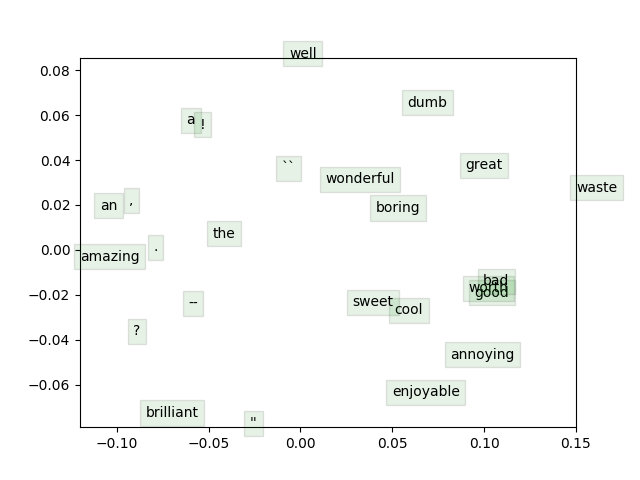
\includegraphics[width=\textwidth]{q3_word_vectors}
  \caption{Visualization of word2vec}\label{fig:1} 
\end{figure}
\paragraph{(h)}See \textbf{q3\_word2vec.py}

\section{Sentiment Analysis}
\paragraph{(a)}See \textbf{q4\_sentiment.py}
\paragraph{(c)}See \textbf{q4\_sentiment.py}
\paragraph{(d)}See \textbf{q4\_sentiment.py}
\paragraph{(e)}See \textbf{q4\_sentiment.py}
\begin{figure}
  \centering
  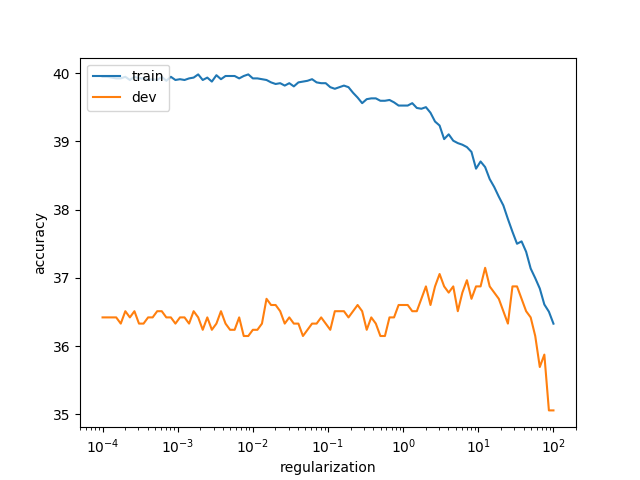
\includegraphics[width=\textwidth]{q4_reg_v_acc}
  \caption{Visualization of word2vec}\label{fig:2} 
\end{figure}

\paragraph{(f)}See \textbf{q4\_sentiment.py}
\begin{figure}
  \centering
  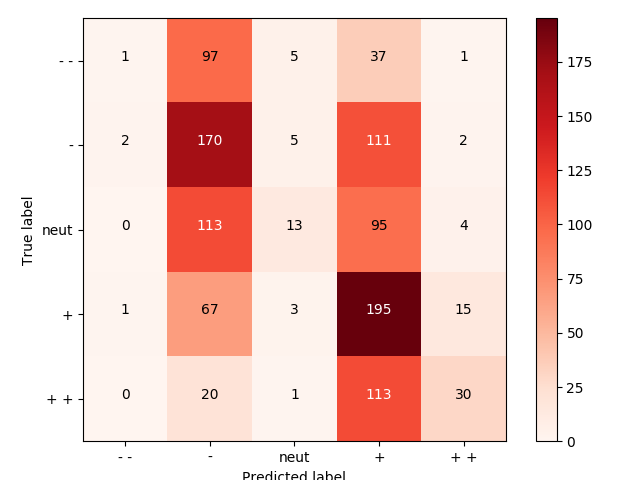
\includegraphics[width=\textwidth]{q4_dev_conf}
  \caption{Visualization of word2vec}\label{fig:3} 
\end{figure}

\paragraph{(g)}
\begin{table}
\centering
\caption{Examples of errors.}\label{Tbl:1}
\begin{tabular}{ |c|c|c| }
  \hline
  True & Pred & Text \\
  \hline
  3 & 1 & and that 's a big part of why we go to the movies. \\
  \hline
  4 & 3 & a quiet treasure -- a film to be savored. \\
  \hline
  1 & 3 & an absurdist comedy about alienation , separation and loss. \\
  \hline
\end{tabular}
\end{table}

\end{spacing}
\end{document}
